\chapter{Fluoride-Salt-Cooled High-Temperature Reactor Benchmark}
\label{chap:fhr-benchmark}
% Main Gist 
% - The work I did for the FHR Benchmark
% Structure 
% - Specifications of benchmark problem
% - Results from benchmark
% Appendix? 
% - More details about the geometry 

The \gls{FHR} is a reactor concept that uses \gls{TRISO} fuel and a 
low-pressure liquid fluoride-salt coolant.
\gls{FHR} technology combines \gls{FLiBe} coolant from \glspl{MSR} and 
\gls{TRISO} particles from \glspl{VHTR} to enable a reactor with 
low operating pressure, large thermal margin, and accident-tolerant 
qualities.
The \gls{AHTR} is a \gls{FHR} type that has plate-based fuel in a hexagonal 
fuel assembly. 
To address the \gls{AHTR} modeling challenges, such as multiple 
heterogeneity and material cross-section data, the \gls{OECD}-\gls{NEA} and 
\gls{Georgia Tech} initiated the \gls{FHR} benchmark for the \gls{AHTR} design 
in 2019 \cite{noauthor_fluoride_nodate}. 
In section \ref{sec:fhr}, I gave an \gls{FHR} concept overview, 
a \gls{AHTR} design description, a review of previous efforts 
towards modeling these designs, and how these efforts led to the benchmark
initiation. 

The \gls{FHR} benchmark has several phases, starting with a single fuel assembly 
simulation without burnup and gradually extending to full core depletion. 
Table \ref{tab:phases} outlines the complete and incomplete benchmark phases.

\begin{table}[H]
    \centering
    \onehalfspacing
    \caption{The \acrlong{FHR} benchmark's Phases \cite{noauthor_fluoride_nodate}.}
	\label{tab:phases}
    \footnotesize
    \begin{tabular}{lclc}
    \hline 
    \textbf{Phases}& \textbf{Sub-phases} & \textbf{Description} & \textbf{Completed?} \\
    \hline
    \multirow{ 3}{5cm}{\textbf{Phase I: fuel assembly (2D/3D with depletion)}} & I-A & 2D model, steady-state (no depletion) & \checkmark\\
    &I-B & 2D model depletion & \checkmark\\
    &I-C & 3D model depletion &\\
    \hline
    \multirow{2}{5cm}{\textbf{Phase II: 3D full core with depletion}}&II-A & Steady-state (no depletion) &\\
    &II-B & Depletion &\\
    \hline 
    \multirow{ 2}{5.5cm}{\textbf{Phase III: 3D full core with feedback \& multicycle analysis}}&III-A & Full core depletion with feedback &\\
    &III-B & Multicycle analysis &\\
    \hline
    \end{tabular}
\end{table}

In the subsequent sections, I will describe the benchmark's specifications for 
the \gls{AHTR} design and Phase I. Then, I will share our Phase I-A and I-B 
results. 

\section{Benchmark Specifications: AHTR Design}
The \acrlong{AHTR} has 3400 MWt thermal power and 1400 MW electric power 
\cite{varma_ahtr_2012}. 
Figure \ref{fig:reactor-schematic} shows the reactor schematic and a vertical 
cut of the reactor vessel. 
\begin{figure}[]
    \centering
    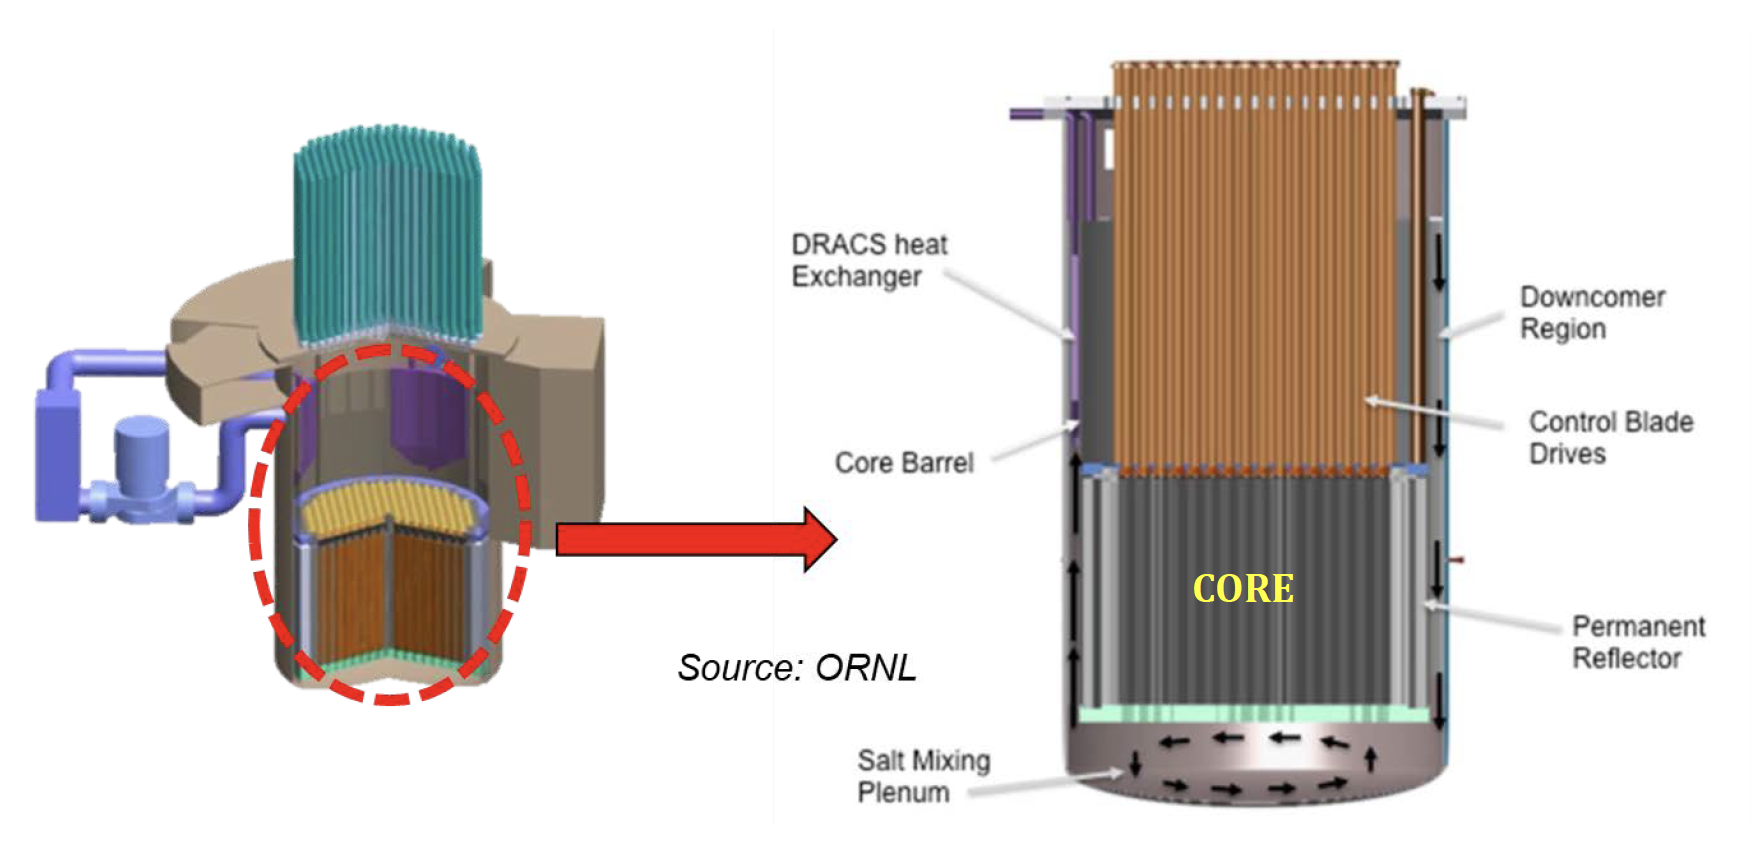
\includegraphics[width=\linewidth]{reactor-schematic.png} 
    \caption{\acrlong{AHTR} schematic (left) and vessel (right) 
    \cite{noauthor_fluoride_nodate}.}
    \label{fig:reactor-schematic}
\end{figure}
Figure \ref{fig:ahtr} shows a single fuel assembly's geometry and all 
assemblies' configuration in the core.
The \gls{AHTR}'s hexagonal fuel assembly detailed 2D view is shown in 
Figure \ref{fig:ahtr-fuel-assembly}.  
\begin{figure}[]
    \centering
    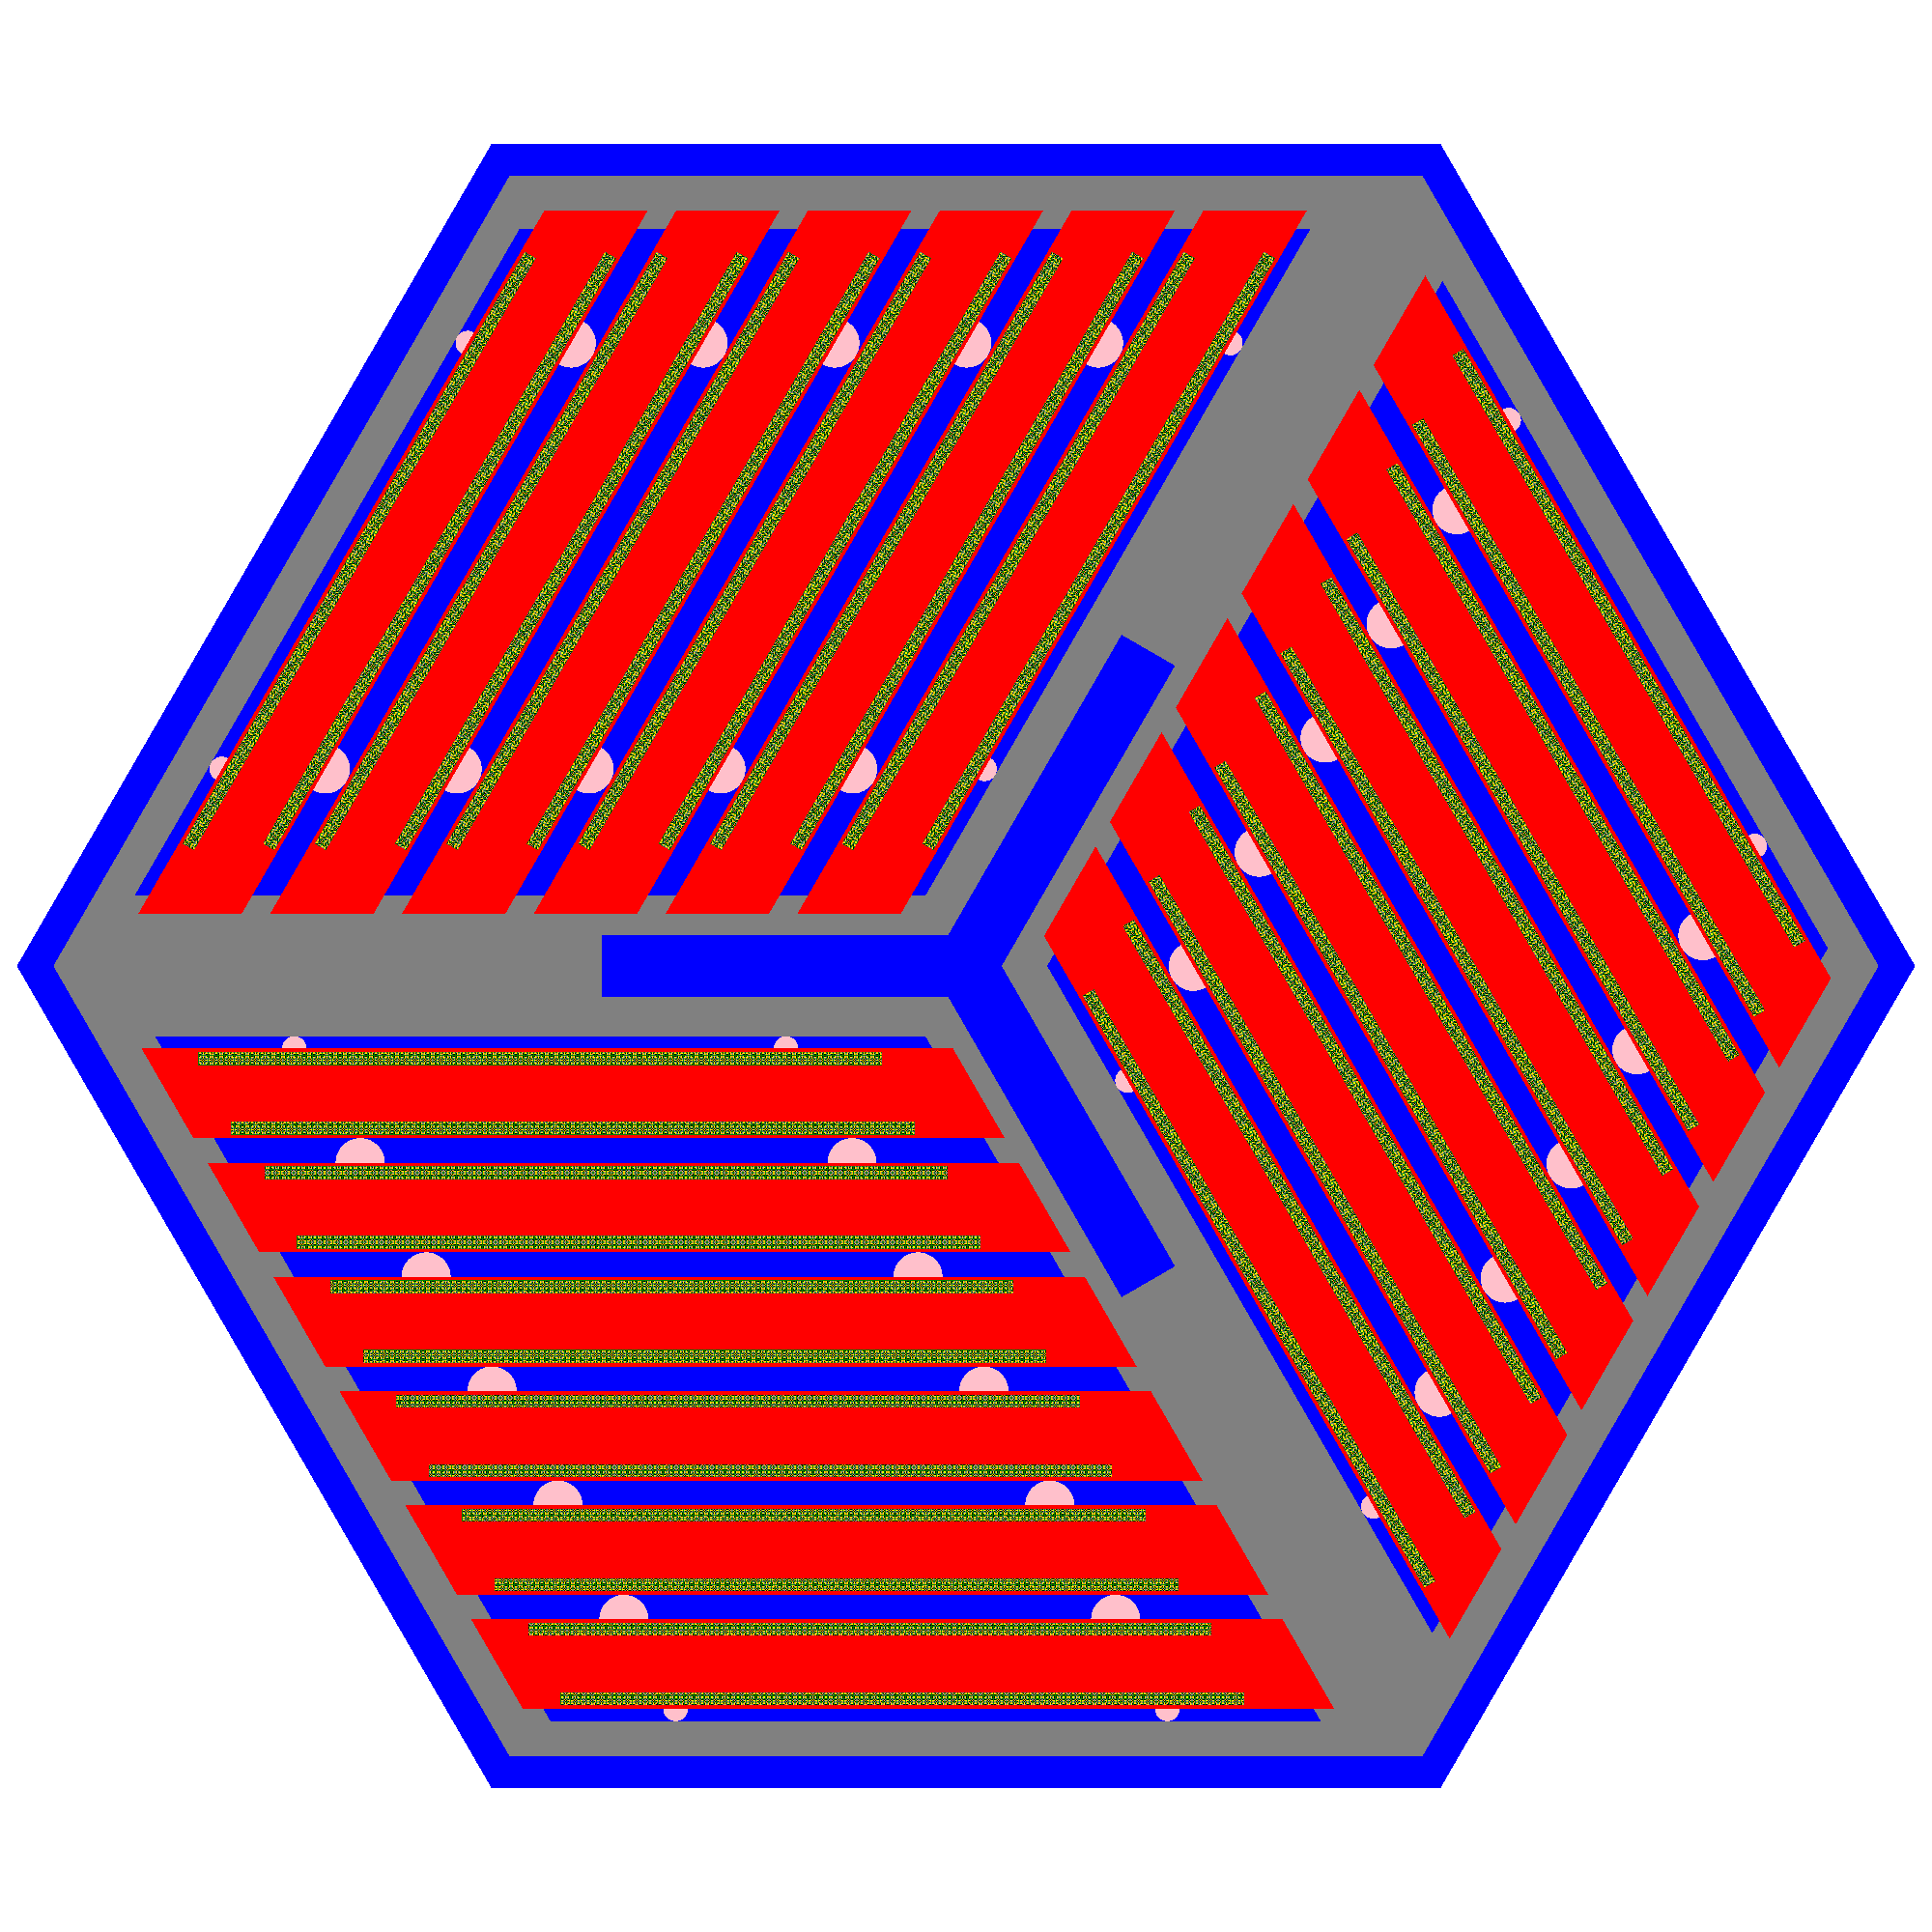
\includegraphics[width=0.7\linewidth]{ahtr-fuel-element.png} 
    \caption{\acrlong{AHTR} fuel assembly with 18 fuel plates arranged in 
    three diamond-shaped sectors, with a central Y-shaped and external channel 
    graphite structure. Blue: FliBE coolant in between fuel assemblies and plates, 
    and in the control rod slot, Gray: graphite structural components, 
    Red: graphite fuel plank, Pink: graphite spacers, Green: graphite matrix 
    with embedded TRISO particles.}
    \label{fig:ahtr-fuel-assembly}
\end{figure}
It features plate-type fuel with hexagonal fuel assembly consisting of eighteen 
planks arranged in three diamond-shaped sectors, with a central Y-shaped 
structure and external channel (wrapper).
The diamond-shaped sections have 120-deg rotational symmetry with each other 
\cite{varma_ahtr_2012,ramey_monte_2018,noauthor_fluoride_nodate}. 
The fuel planks have semi-cylindrical spacers attached, their radius being 
equal to the coolant channel thickness. 

Figure \ref{fig:y-shape} shows the external channel wrapper and structural 
Y-shape, which are made of C-C composite and have extra notches to hold 
the fuel plates in place.
\begin{figure}[]
    \centering
    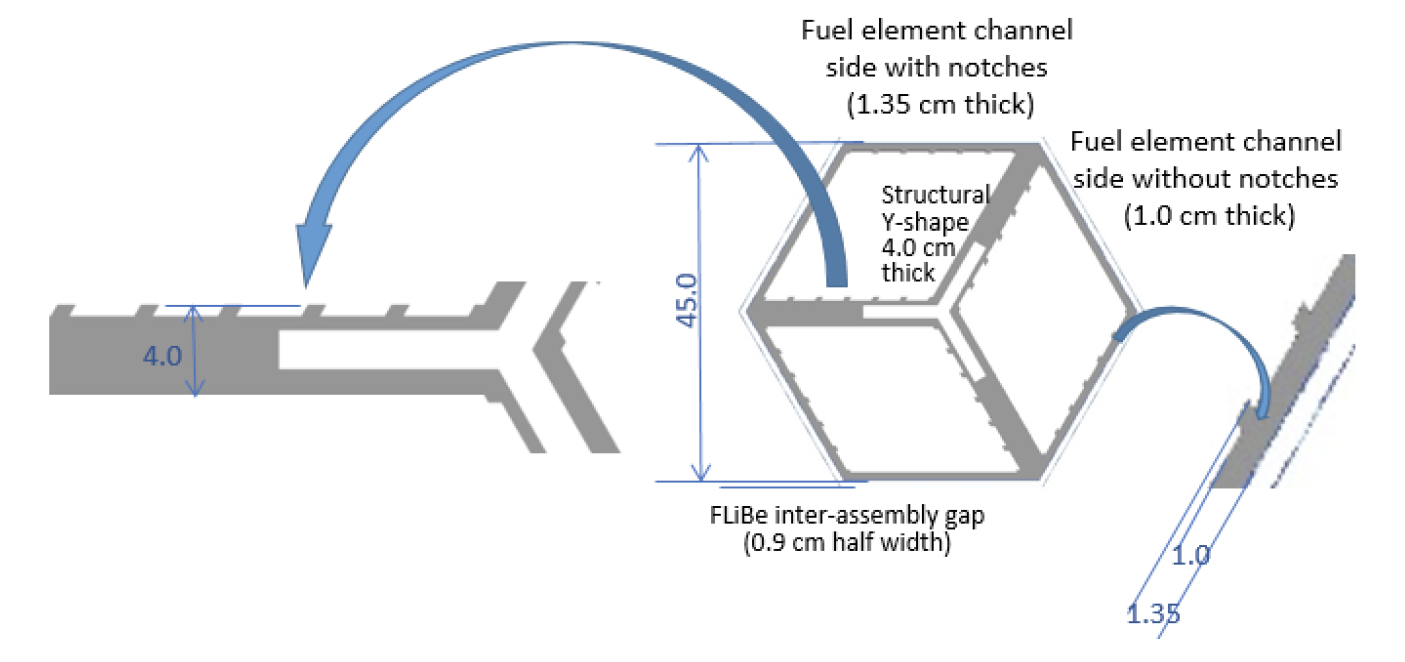
\includegraphics[width=\linewidth]{y-shape.png} 
    \caption{\acrlong{AHTR} fuel assembly's structural components 
    \cite{noauthor_fluoride_nodate}.}
    \label{fig:y-shape}
\end{figure}
The gap between the fuel assemblies and fuel plates is filled with \gls{FLiBe}
coolant. 
The Y-shaped control rod slot at the center of the Y-shape structure contains 
\gls{FLiBe} coolant when the control blade is not in the slot (as seen in 
Figure \ref{fig:ahtr-fuel-assembly})
\cite{varma_ahtr_2012,ramey_monte_2018,noauthor_fluoride_nodate}.
Each fuel plank is made of an isostatically pressed carbon with fuel stripes 
on each outer side of the plank, as seen in Figure \ref{fig:ahtr-fuel-plank}. 
\begin{figure}[]
    \centering
    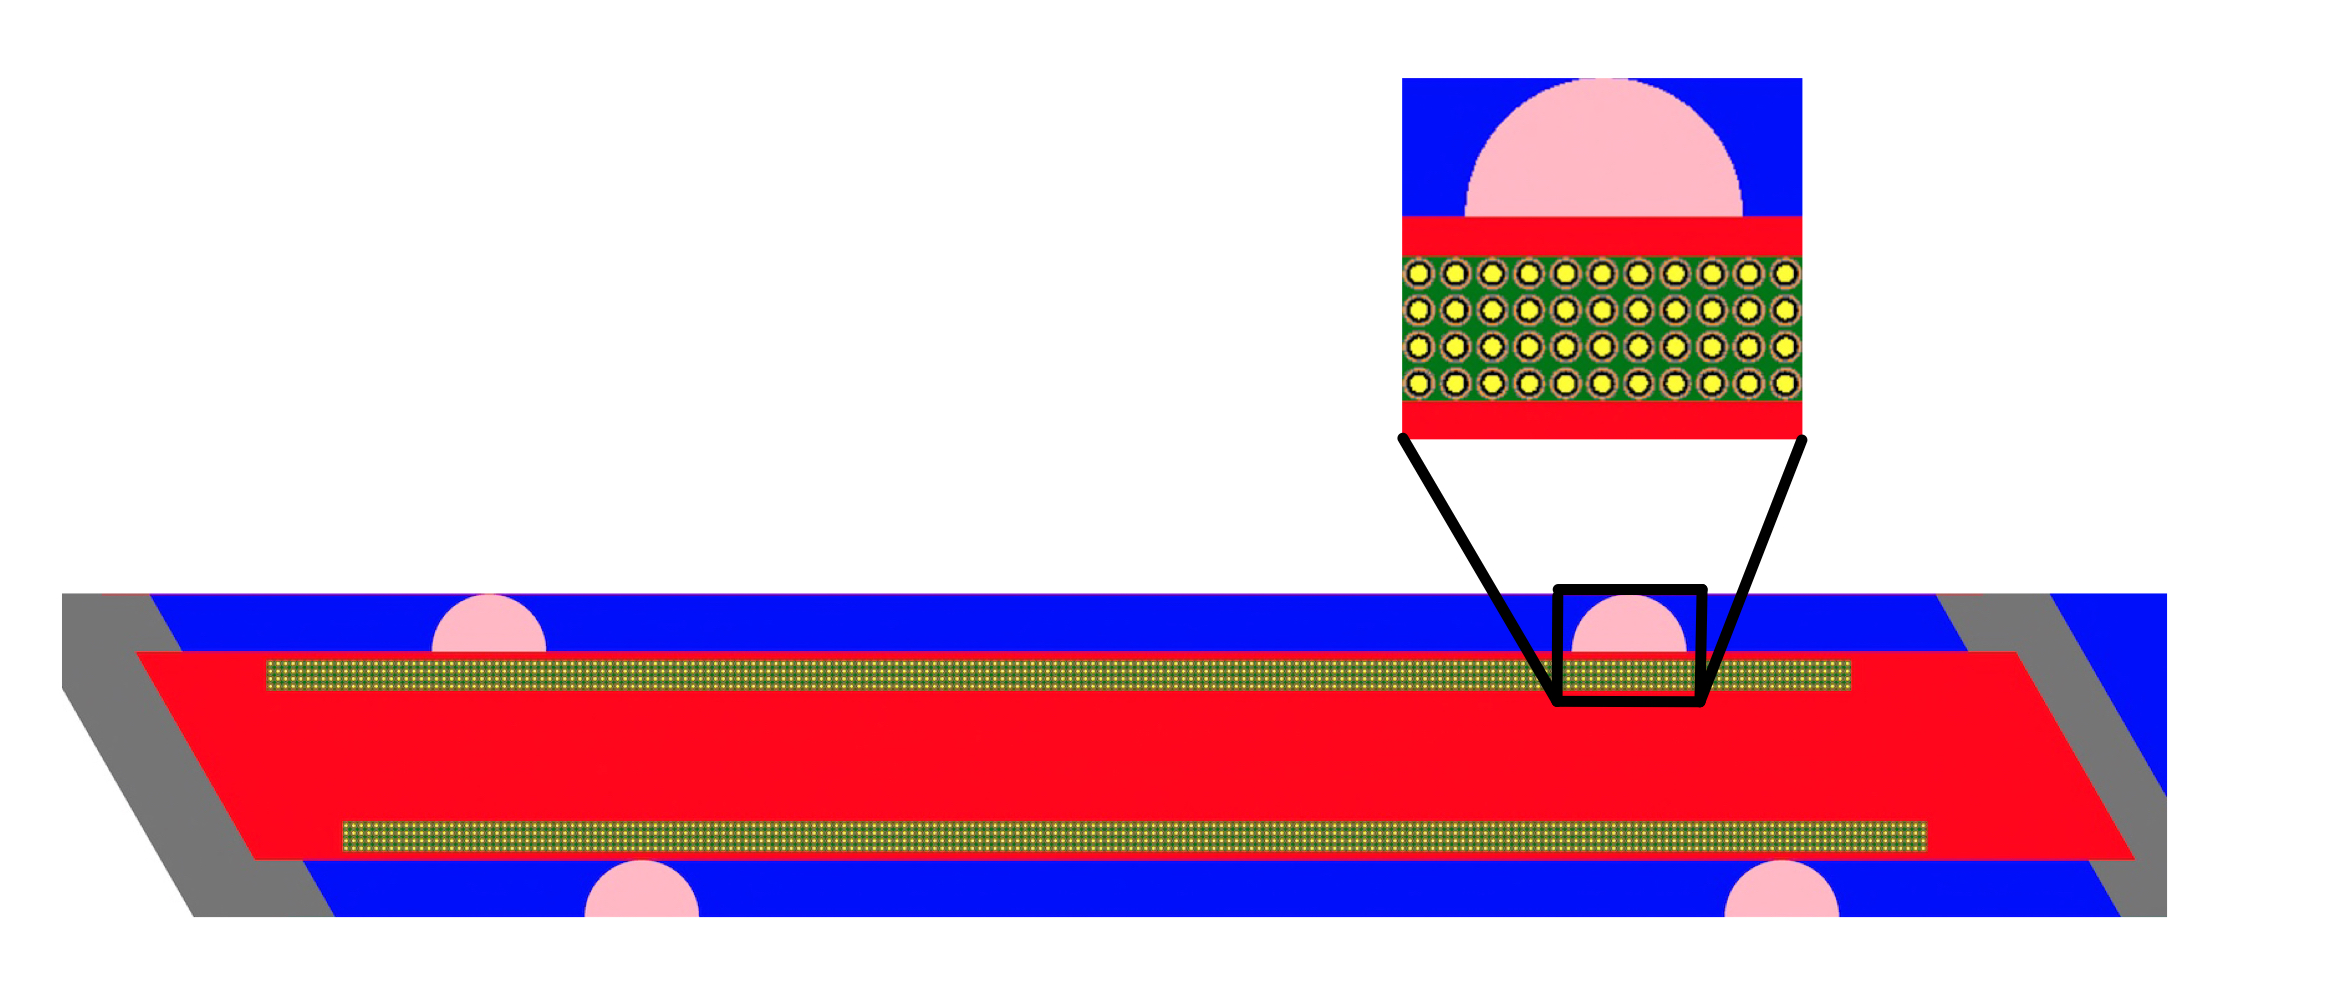
\includegraphics[width=\linewidth]{ahtr-fuel-plank.png} 
    \caption{\acrlong{AHTR}'s fuel plank, with the magnification of 
    a spacer and segment of the fuel stripe with embedded TRISO particles.}
    \label{fig:ahtr-fuel-plank}
\end{figure}
The fuel stripes are prismatic regions composed of a graphite matrix filled with 
a cubic lattice of \gls{TRISO} particles with a 40\% packing fraction. 
The lattice is 210 \gls{TRISO} particles wide in the x-direction, four particles 
deep in the y-direction, and 5936 particles tall in the z-direction. 
Each \gls{TRISO} particle has five layers (Figure \ref{fig:ahtr-triso}): 
oxycarbide fuel kernel, porous carbon buffer, inner pyrolytic carbon, silicon 
carbide layer, and the outer pyrolitic carbon. 
\begin{figure}[]
    \centering
    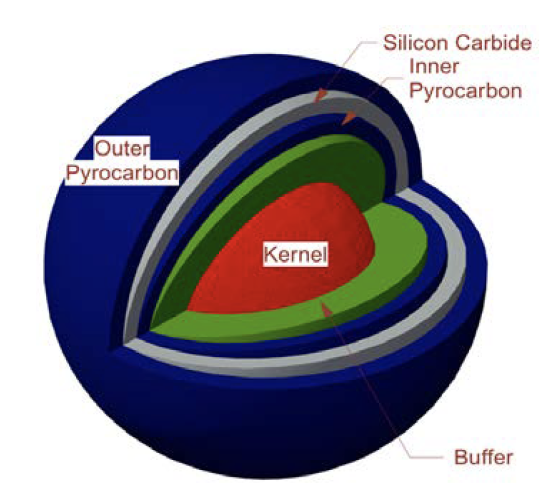
\includegraphics[width=0.6\linewidth]{ahtr-triso.png} 
    \caption{\acrlong{AHTR}'s TRISO particle schematic \cite{noauthor_fluoride_nodate}.}
    \label{fig:ahtr-triso}
\end{figure}

For reactivity control, burnable poisons and control rods are included in 
some configurations of the \gls{AHTR}. 
The burnable poisons consist of europium oxide, $Eu_2O_3$, and have a discrete
or integral (dispersed) option. 
In the discrete option, small spherical $Eu_2O_3$ particles are stacked axially 
at five locations in each fuel plank, as shown in Figure \ref{fig:discrete-poison}. 
\begin{figure}[]
    \centering
    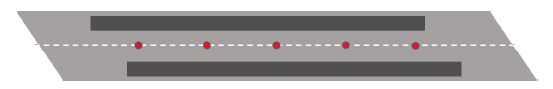
\includegraphics[width=\linewidth]{discrete-poison.png} 
    \caption{Placement of axial stacks of burnable poisons in the \acrlong{AHTR} 
    \cite{noauthor_fluoride_nodate}.}
    \label{fig:discrete-poison}
\end{figure}
In the integral option, $Eu_2O_3$ is homogenously mixed with the fuel plank 
graphite matrix (including the graphite in fuel stripes matrix and plank ends 
indented to structural sides, but excluding the graphite in spacers and 
graphite in TRISO particles). 
Each control rod is uniformly composed of \gls{MHC} and is inserted into the 
Y-shaped control rod slot where it displaces the \gls{FLiBe} that occupies the 
slot (Figure \ref{fig:ahtr-fuel-assembly}). 

\section{Benchmark Specifications: Phase I}
\label{sec:phase1}
The \gls{FHR} benchmark's Phase I consists of a steady-state 2D model 
(Phase I-A) and depletion (Phase I-B) of one \gls{FHR} fuel assembly. 
For a single fuel assembly, the internal 120-degree rotational symmetry is 
represented by periodic boundary conditions, as seen in Figure \ref{fig:bc}. 
\begin{figure}[]
    \centering
    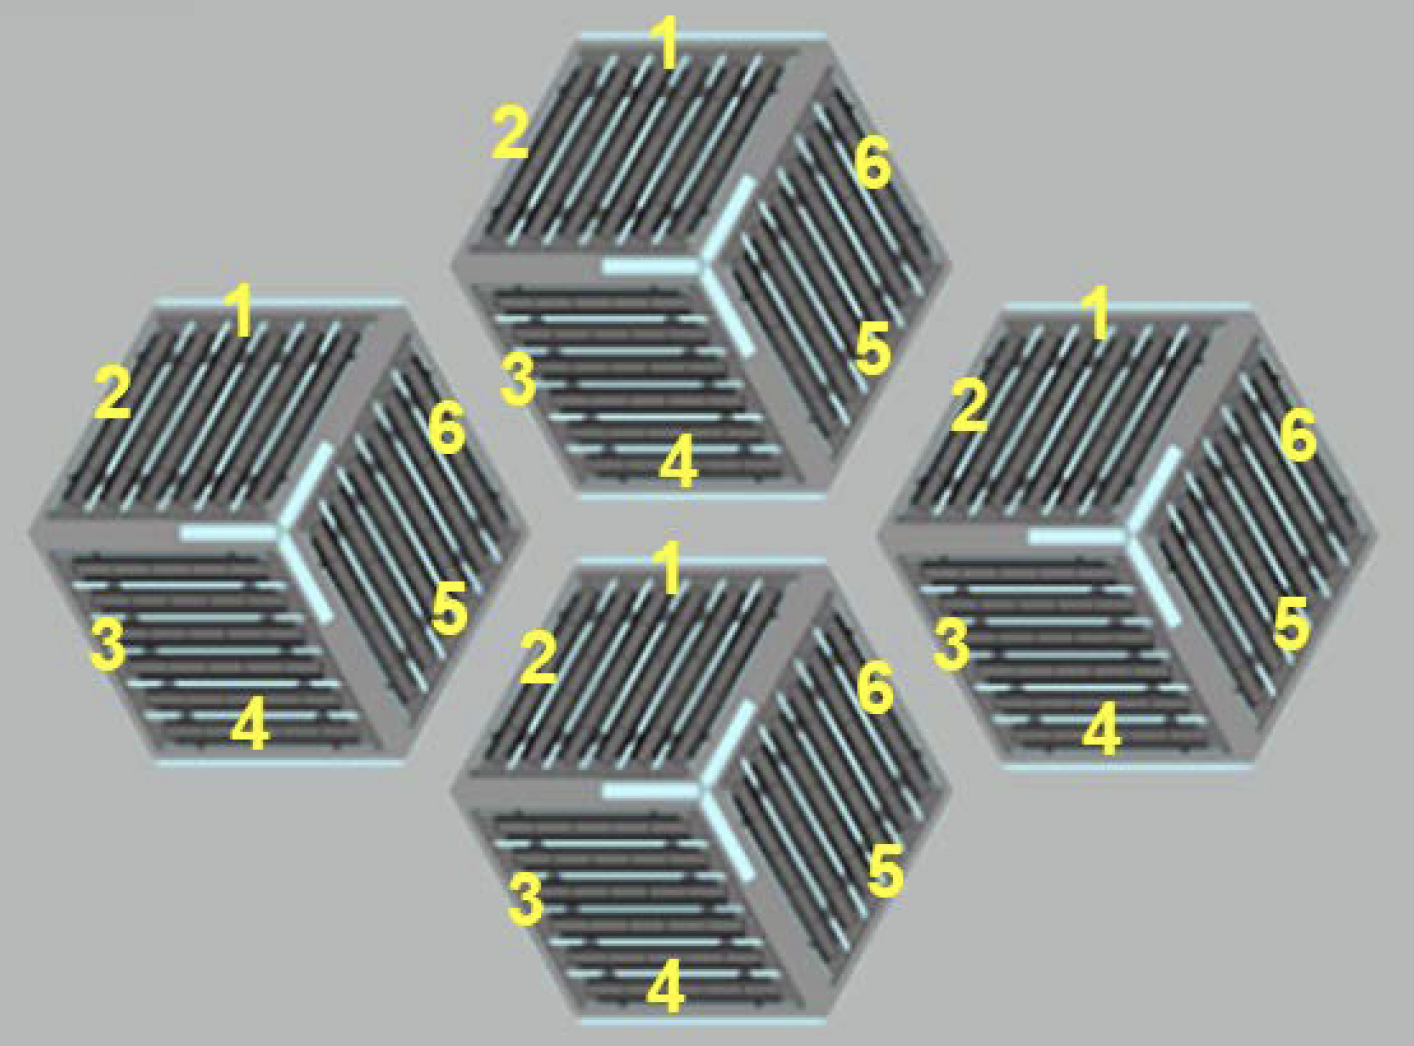
\includegraphics[width=0.7\linewidth]{bc.png} 
    \caption{Visualization of periodic boundary conditions for a single fuel 
    assembly in the \gls{AHTR}\cite{noauthor_fluoride_nodate}.}
    \label{fig:bc}
\end{figure}
The benchmark required the following results for Phases I-A and I-B:
\begin{enumerate}[label=(\alph*)]
    \item effective multiplication factor 
    \item reactivity coefficients ($\beta_{eff}$, fuel Doppler coefficient, FLiBe 
    temperature coefficient, graphite temperature coefficient)
    \item tabulated fission source distribution by one-fifth fuel stripe
    \item neutron flux averaged over the whole model tabulated in three coarse energy groups
    \item neutron flux distribution in three coarse energy groups
    \item fuel assembly averaged neutron spectrum
\end{enumerate}
Next, I report the equations used to calculate these required results.  

\subsubsection{Reactivity Coefficients (b)}
Effective delayed neutron fraction ($\beta_{eff}$) is the fraction of delayed 
neutrons in the core. 
I assumed one energy group and six delayed groups for $\beta_{eff}$. 
Reactivity coefficient is the change in reactivity ($\rho$) of the material 
per degree change in the material's temperature (T). 
I calculated each reactivity coefficient and its corresponding uncertainty 
with these equations: 
\begin{align}
    \frac{\Delta \rho}{\Delta T} &= 
    \frac{\rho_{T_{high}}-\rho_{T_{low}}}{T_{high}-T_{low}} \ [\frac{pcm}{K}] \\
    \delta \frac{\Delta \rho}{\Delta T} &= 
    \frac{\sqrt{\delta (\rho_{T_{high}})^2+(\delta \rho_{T_{low}})^2}}{T_{high}-T_{low}} \ [\frac{pcm}{K}] 
\end{align}

\subsubsection{Fission Source Distribution / Fission Density (c)}
I calculated \gls{FD} with OpenMC's \texttt{fission} tally score (f) 
for each region divided by the average \texttt{fission} tally score of all the regions:
\begin{align}
    FD_i &=  \frac{f_i}{f_{ave}} \\
    \intertext{where}
    f_i &= \mbox{fission reaction rate in a single region [reactions/src]} \nonumber \\
    f_{ave} &= \mbox{average of all $f_i$ [reactions/src]} \nonumber
\end{align}
The uncertainty calculations for $FD_i$ and $f_{ave}$: 
\begin{align}
    \delta FD_i &= |FD_i| \sqrt{(\frac{\delta f_i}{f_i})^2+(\frac{\delta f_{ave}}{f_{ave}})^2} \\
    \delta f_{ave} &= \frac{1}{N}\sqrt{\sum_i^Nf_i^2} \\
    \intertext{where}
    N &= \mbox{No. of fission score values} \nonumber
\end{align}

\subsubsection{Neutron Flux (d, e, f)}
OpenMC's \texttt{flux} score is in [$\frac{neutrons\ cm}{src}$] units. 
For the benchmark, I converted flux to [$\frac{neutrons}{cm^2s}$] units
using the following equations:  

\begin{align}
    \Phi_c &= \frac{N \times \Phi_o}{V} \\
    N &= \frac{P\times\nu}{Q\times k} \\
    \intertext{where}
    \Phi_c &= \mbox{converted flux [$\frac{neutrons}{cm^2s}$]} \nonumber \\ 
    \Phi_o &= \mbox{original flux [$\frac{neutrons\ cm}{src}$]} \nonumber \\
    N &= \mbox{normalization factor [$\frac{src}{s}$]} \nonumber \\
    V &= \mbox{volume of fuel assembly [$cm^3$]} \nonumber \\
    P &= \mbox{power [$\frac{J}{s}$]} \nonumber \\
    \nu &= \mbox{$\frac{\nu_f}{f}$ [$\frac{neutrons}{fission}$]} \nonumber \\
    Q &= \mbox{Energy produced per fission [$\frac{J}{fission}$]} = \mbox{$3.2044 \times 10^{-11}$ J per $U_{235}$ fission} \nonumber \\
    k &= \mbox{$k_{eff}$ [$\frac{neutrons}{src}$]} \nonumber 
\end{align}
The flux standard deviation is: 
\begin{align}
    \delta \Phi_c = \Phi_c \times
    \sqrt{(\frac{\delta \Phi_o}{\Phi_o})^2+ (\frac{\delta \nu_f}{\nu_f})^2 
    + (\frac{\delta k}{k})^2 + (\frac{\delta f}{f})^2}
\end{align}
I calculated reactor power based on the given reference specific power 
($P_{sp}$) of 200 $\frac{W}{gU}$: 
\begin{align}
    P &= P_{sp} \times V_F \times \rho_F \times \frac{wt\%_{U}}{100} \\
    \intertext{where}
    V_F &= \mbox{volume of fuel [$cm^3$]} = \frac{4}{3} \pi r_f^3 \times N_{total} \nonumber \\
    r_f &= \mbox{radius of fuel kernel} \nonumber\\
    N_{total} &= \mbox{total no. of TRISO particles in fuel assembly} = 101 \times 210 \times 4 \times 2 \times 6 \times 3 \nonumber\\ 
    \rho_F &= \mbox{density of fuel [$g/cc$]} \nonumber \\
    wt\%_{U} &= \frac{at\%_{U235} \times AM_{U235} + at\%_{U238} \times AM_{U238}}{\sum (at\%_i \times AM_i)} \times 100 \nonumber\\
    AM &= \mbox{atomic mass} \nonumber
\end{align}

\subsection{Benchmark Specifications: Phase I-A}
For Phase I-A, the benchmark specifies that each participant must produce a 
steady-state 2D model of one fresh fuel assembly for nine cases
and report the required results listed in Section \ref{sec:phase1}.  
Table \ref{tab:phase1a-cases} describes each case. 
\begin{table}[H]
    \centering
    \onehalfspacing
    \caption{Description of the \acrlong{FHR} benchmark Phase I-A cases \cite{noauthor_fluoride_nodate}.}
	\label{tab:phase1a-cases}
    \footnotesize
    \begin{tabular}{p{0.05\textwidth}|p{0.95\textwidth}}
    \hline 
    \textbf{Case} & \textbf{Description} \\
    \hline
    1A & Reference case. Hot full power (HFP), with temperatures of 1110K for 
    fuel kernel and 948K for coolant and all other materials (including TRISO 
    particle layers other than fuel kernel). Nominal (cold) dimensions, 
    9 wt\% enrichment, no \gls{BP}, \glspl{CR} out.\\
    \hline
    2AH & \Gls{HZP} with uniform temperature of 948 K, 
    otherwise same as Case 1A. Comparison with Case 1A provides HZP-to-HFP power 
    defect.\\
    \hline 
    2AC & \Gls{CZP}. Same as Case 2AH, but with uniform temperature 
    of 773 K. Comparison with Case 2AH provides isothermal temperature coefficient.\\
    \hline
    3A & \gls{CR} inserted, otherwise same as Case 1A. \\
    \hline
    4A & Discrete europia \gls{BP}, otherwise same as Case 1A.\\
    \hline
    4AR & Discrete europia \gls{BP} and \gls{CR} inserted, otherwise same as 
    Case 1A. \\
    \hline
    5A & Integral (dispersed) europia \gls{BP}, otherwise same as Case 1A. \\
    \hline
    6A & Increased \gls{HM} loading (4 to 8 layers of \gls{TRISO}) decreased C/HM 
    ratio (from about 400 to about 200) and decreased specific power to 100 W/gU, 
    otherwise same as Case 1A.\\
    \hline 
    7A & Fuel enrichment 19.75 wt\%, otherwise same as Case 1A.\\
    \hline 
    \end{tabular}
\end{table}

\subsection{Benchmark Specifications: Phase I-B}
For Phase I-B, the benchmark specifies that each participant must produce 
depletion results for three cases: 1B, 4B, and 7B. 
These are the same as cases 1A, 4A, and 7A, but with depletion steps added. 
The benchmark assumes that depletion occurs only in the fuel and \glspl{BP} and 
that the depletion performs under the critical spectrum assumption. 

\section{Results}
Several organizations participated in the benchmark with various Monte Carlo
and Deterministic neutronics codes, such as Serpent \cite{leppanen_serpent_2014}, 
OpenMC \cite{romano_openmc_2013}, and WIMS \cite{lindley_current_2017}. 
\gls{UIUC} participated in the benchmark with the OpenMC Monte Carlo code 
\cite{romano_openmc_2013} and the ENDF/B-VII.1 material library 
\cite{chadwick_endf/b-vii.1_2011}.
The \texttt{fhr-benchmark} Github repository contains all the results submitted 
by \gls{UIUC} for the \gls{FHR} benchmark \cite{chee_arfcfhr-benchmark_2021}. 
The benchmark used a phased blind approach -- participants were asked to 
submit Phase I-A and I-B results without knowledge of other submissions. 
Petrovic et al. \cite{petrovic_preliminary_2021} describes the preliminary 
results of the benchmark results across several institutions and concludes 
that the overall observed agreement is satisfactory. 
In the subsequent sections, I will share the results obtained by \gls{UIUC}.  

\subsection{Results: Phase I-A}
Petrovic et al. \cite{petrovic_preliminary_2021} compared the effective 
multiplication factor ($k_{eff}$) for all participants and Phase I-A cases in 
the \gls{FHR} benchmark. 
They reported that the standard deviation between participants for each case 
was in the 231 to 514 pcm range, acceptable and notably close given a blind 
benchmark, assuring us that our Phase I-A results are acceptable and in agreement 
with other benchmark participants. 

Table \ref{tab:phase1a-cases} reports Phase I-A $k_{eff}$ and reactivity 
coefficients results. 
I ran the simulations on \gls{UIUC}'s BlueWaters supercomputer with 64 XE nodes, 
which each have 32 cores \cite{ncsa_about_2017}. 
To reduce $k_{eff}$'s statistical uncertainty to $\sim$10pcm, I ran each simulation 
with 500 active cycles, 100 inactive cycles, and 200000 neutrons. 
Each simulation took \gls{WCT} ranging from 2 to 5 hours. 
\begin{table}[H]
    \centering
    \onehalfspacing
    \caption{\acrlong{UIUC}'s \acrlong{FHR} Benchmark Phase I-A results 
    \cite{chee_arfcfhr-benchmark_2021}.}
	\label{tab:phase1a-results}
    \footnotesize
    \begin{tabular}{cp{2.7cm}cccccc}
    \hline
    \textbf{Case} & \textbf{Summary} & \textbf{WCT [hr]} & \textbf{$k_{eff}$}* & 
    \textbf{$\beta_{eff}$}** & 
    \textbf{Fuel} $\frac{\Delta \rho}{\Delta T}$ & 
    \textbf{FliBe} $\frac{\Delta \rho}{\Delta T}$ & 
    \textbf{Graphite} $\frac{\Delta \rho}{\Delta T}$\\
    \hline 
    1A & Reference &2.82&1.39389 & 0.006534 & -2.24$\pm$0.15 & -0.15$\pm$0.15 & -0.68$\pm$0.15\\
    2AH & \gls{HZP} &2.82&1.40395 & 0.006534 & -3.14$\pm$0.15 & -0.20$\pm$0.14 & -0.85$\pm$0.14\\
    2AC & \gls{CZP} &2.75&1.41891 & 0.006534 & -3.36$\pm$0.14 & -0.11$\pm$0.14 & 0.07$\pm$0.14\\
    3A & \gls{CR} &2.49&1.03147 & 0.006534 & -4.03$\pm$0.28 & -0.83$\pm$0.27 & -3.18$\pm$0.29\\
    4A & Discrete \gls{BP} &5.08&1.09766 & 0.006542 & -4.06$\pm$0.24 & -1.55$\pm$0.23 & -6.51$\pm$0.24\\
    4AR & Discrete \gls{BP} + \gls{CR} &4.59&0.84158 & 0.006553 & -5.60$\pm$0.49 & -1.78$\pm$0.46 & -10.44$\pm$0.47\\
    5A & Dispersed \gls{BP} &2.33&0.79837 & 0.006556 & -5.09$\pm$0.40 & -4.87$\pm$0.40 & -22.99$\pm$0.38\\
    6A & Increased \gls{HM} &3.52&1.26294 & 0.006556 & -4.46$\pm$0.19 & 0.16$\pm$0.20 & -0.39$\pm$0.20\\
    7A & 19.75\% Enriched &2.21&1.50526 & 0.006530 & -2.49$\pm$0.13 & -0.12$\pm$0.12 & -0.62$\pm$0.12\\
    \hline
    \multicolumn{5}{l}{* All $k_{eff}$ values have an uncertainty of 0.00010.} \\
    \multicolumn{5}{l}{** All $\beta_{eff}$ values have an uncertainty of 0.000001.} 
    \end{tabular}
\end{table}

Cases 2AH and 2AC are at zero power, meaning that the fuel assembly is exactly 
critical but not producing any energy. 
For both cases, $k_{eff}$ is higher than the reference Case 1A, which I attribute to 
lower fuel temperatures. 
At lower fuel temperatures, less doppler broadening occurs, 
resulting in less neutron capture, thus, increasing $k_{eff}$. 
As expected, $k_{eff}$ is lower for Cases 3A, 4AR, and 5A than reference case 
1A since these cases introduce burnable poisons and control rods to the fuel 
assembly. 
Also, as expected, $k_{eff}$ is higher for Case 7A than reference Case 1A, since 
it has a higher enrichment. 
However, Case 6A deviated from expectations with a lower $k_{eff}$ despite an increase 
in \acrlong{HM} loading. 
This behavior is due to reduced moderation and worsened fuel 
utilization brought about by self-shielding, demonstrating that an increase in 
fuel packing fraction does not always correspond with an increased $k_{eff}$. 

$\beta_{eff}$ increased by 10-20pcm for Cases 4A, 4AR, 5A, and 6A compared to
reference Case 1A due to the introduction of control rods and poisons that 
shift the average neutron velocity to higher values, resulting in decreased
thermal fission and increased fast fission \cite{torabi_neutronic_2018}.
Table \ref{tab:phase1a-results} reports that most of the temperature coefficients 
are negative, exemplifying the \gls{AHTR}'s passive safety behavior. 
Negative reactivity feedback results in a self-regulating reactor; if the reactor's 
power rises, resulting in temperature increase, the negative reactivity
reduces power. 

Figure \ref{fig:phase1a-c} shows the fission source distribution by 
one-fifth fuel stripe for Cases 1A and 3A. 
\begin{figure}[]
    \centering
    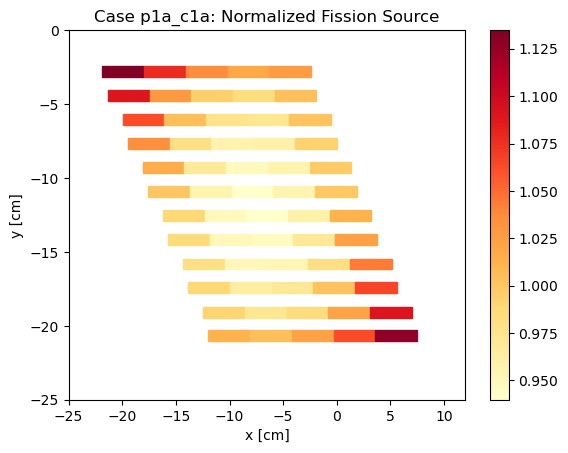
\includegraphics[width=0.49\linewidth]{p1a_c1a_c.png} 
    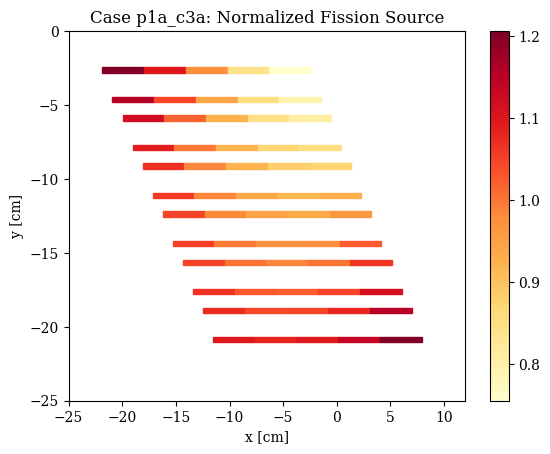
\includegraphics[width=0.48\linewidth]{p1a_c3a_c.png} 
    \caption{Fission Source Distribution per one-fifth fuel stripe for \acrlong{FHR} 
    Benchmark's Phase I-A Case 1A (left) and Case 3A (right).}
    \label{fig:phase1a-c}
\end{figure}
Case 4AR has a similar fission source distribution as Case 3A since both 
cases have control rod insertion. 
All other cases have similar fission source distributions to Case 1A. 
For Case 1A, intuitively, I would assume that the highest fission source would 
occur in the center of the diamond fuel segment; however, the opposite is true. 
Power peaking occurs on exterior stripes and is minimum on the interior stripes.
Gentry et al. \cite{gentry_development_2016} reported similar power peaking 
phenomena towards the lattice cell's exterior closest to the Y-shaped carbon 
support structure where the thermal flux is most elevated. 
The lowest power is found in the interiors of the lattice tri-sections. 
This fission source distribution is caused by diminished resonance escape 
probability in the interior due to the higher relative fuel-to-carbon volume 
ratio. 
Cases 6A and 7A demonstrate a further diminished fission source in the interior 
stripes due to the higher fuel-to-carbon ratio.
For Case 3A with an inserted control rod, the fission source is lower in 
the one-fifth stripes closer to the control rod.  

Figure \ref{fig:phase1a-d} shows the average neutron flux in the fuel assembly in 
three coarse energy groups. 
\begin{figure}[]
    \centering
    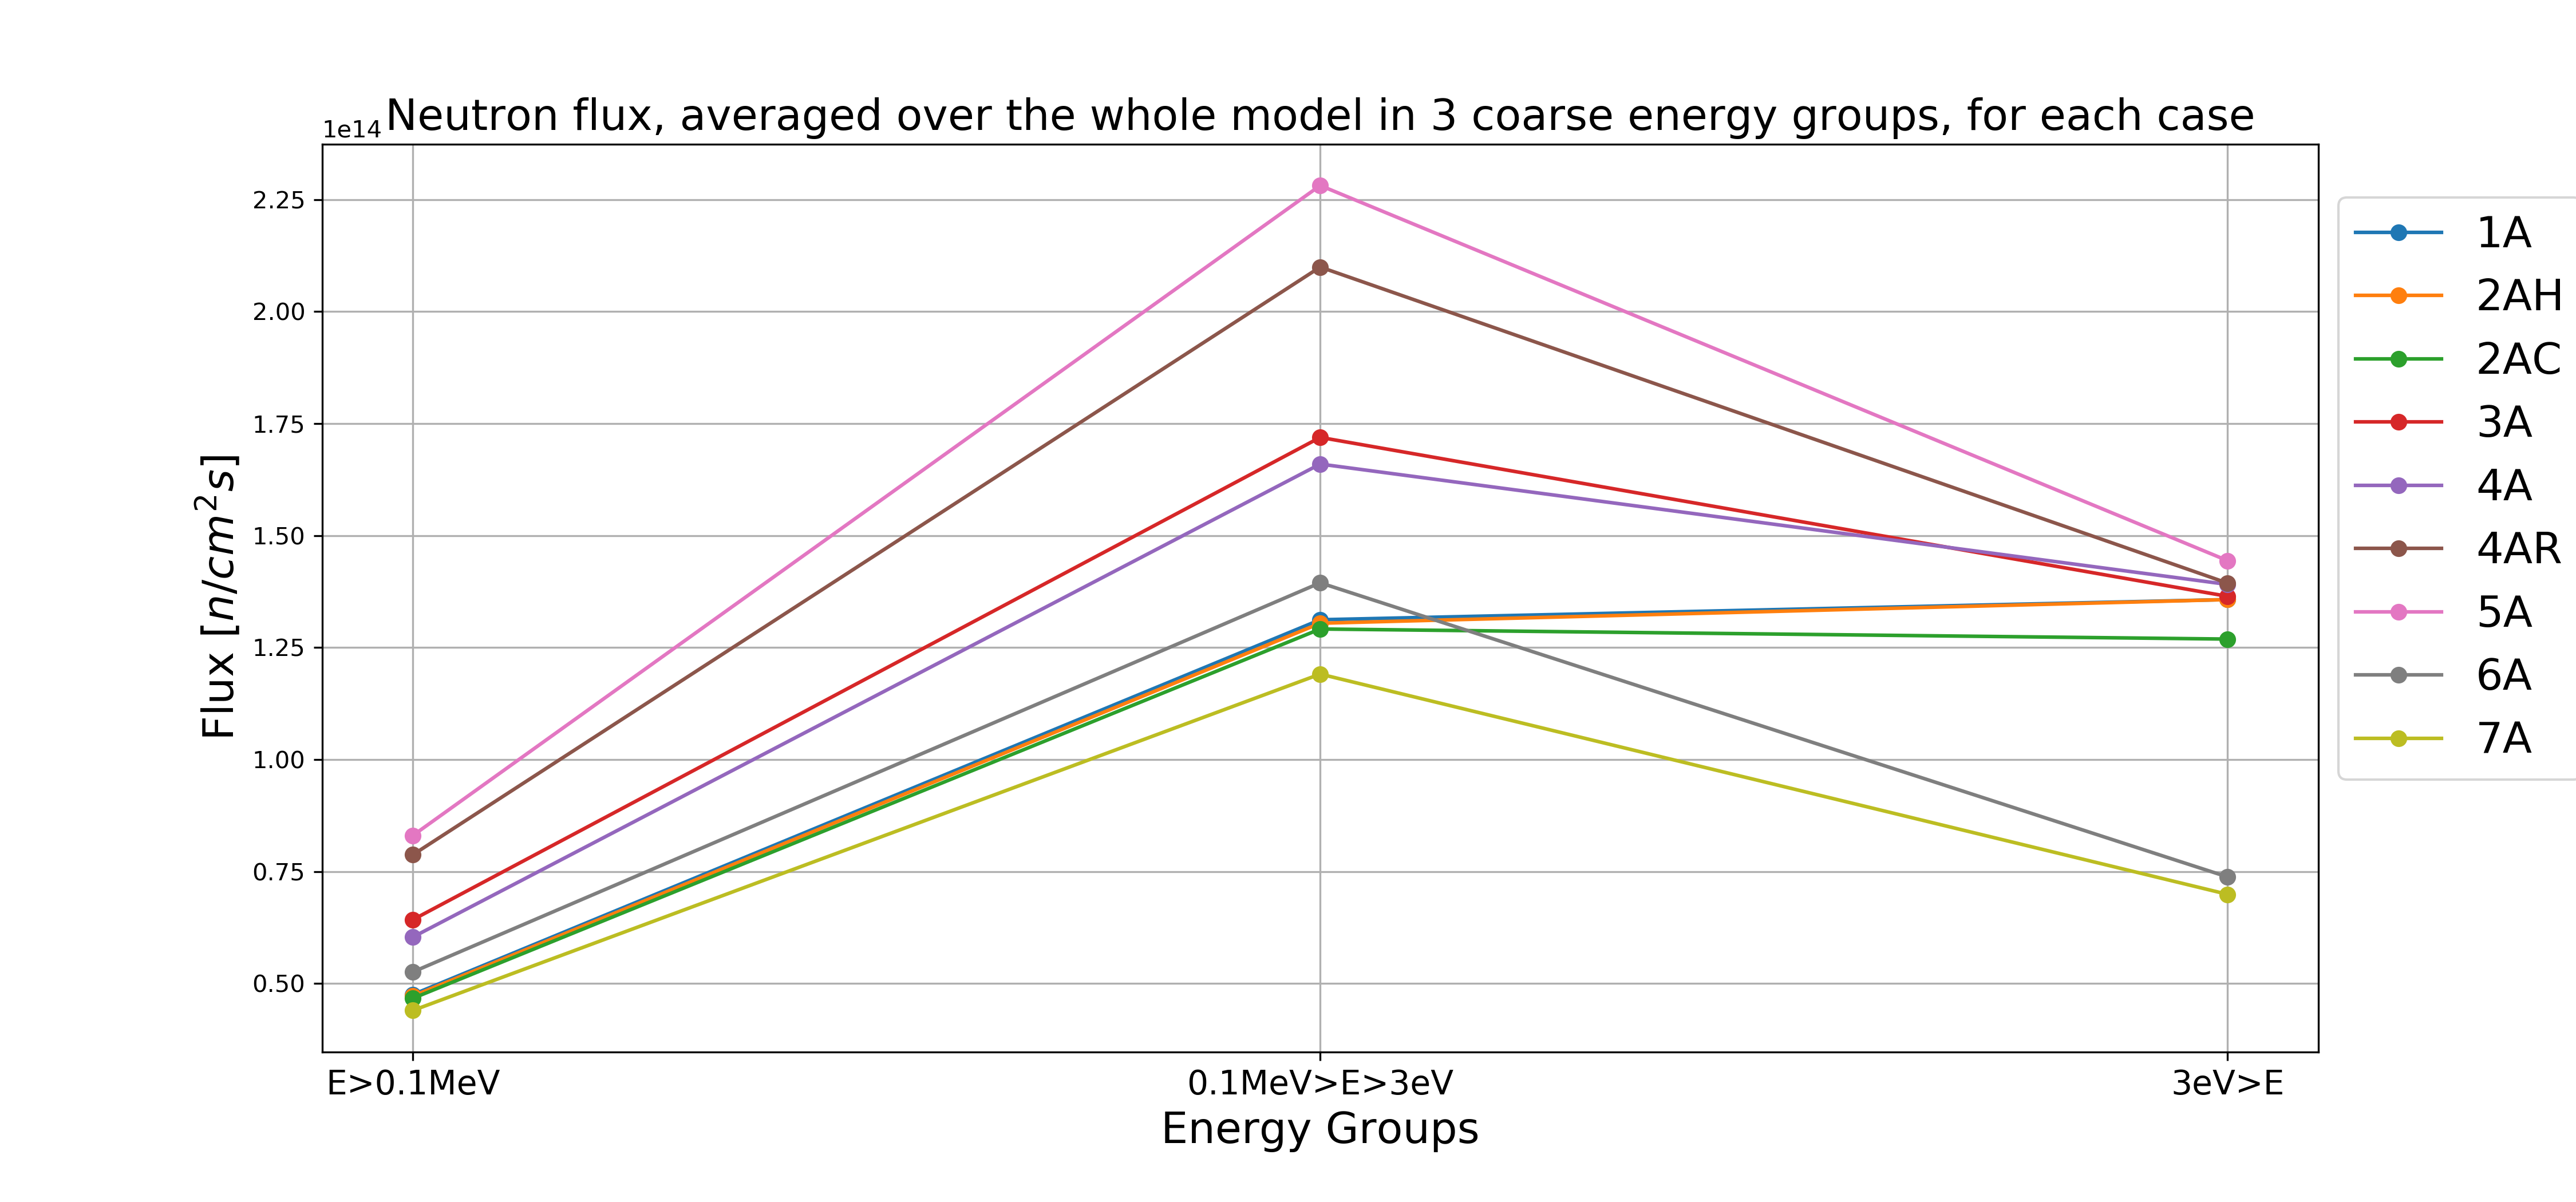
\includegraphics[width=\linewidth]{phase1a-d-flux.png} 
    \caption{\acrlong{FHR} Benchmark's Neutron flux, averaged over the whole 
    model, tabulated in three coarse energy groups for each Phase I-A case. }
    \label{fig:phase1a-d}
\end{figure}
Most of the cases have the most flux in the intermediate group, followed by 
the thermal group, and the least flux in the fast group.    
Figure \ref{fig:phase1a-e} shows the neutron flux distribution in a 100 $\times$ 
100 mesh for Cases 1A, 3A, and 6A for three coarse energy groups. 
\begin{figure}[]
    \centering
    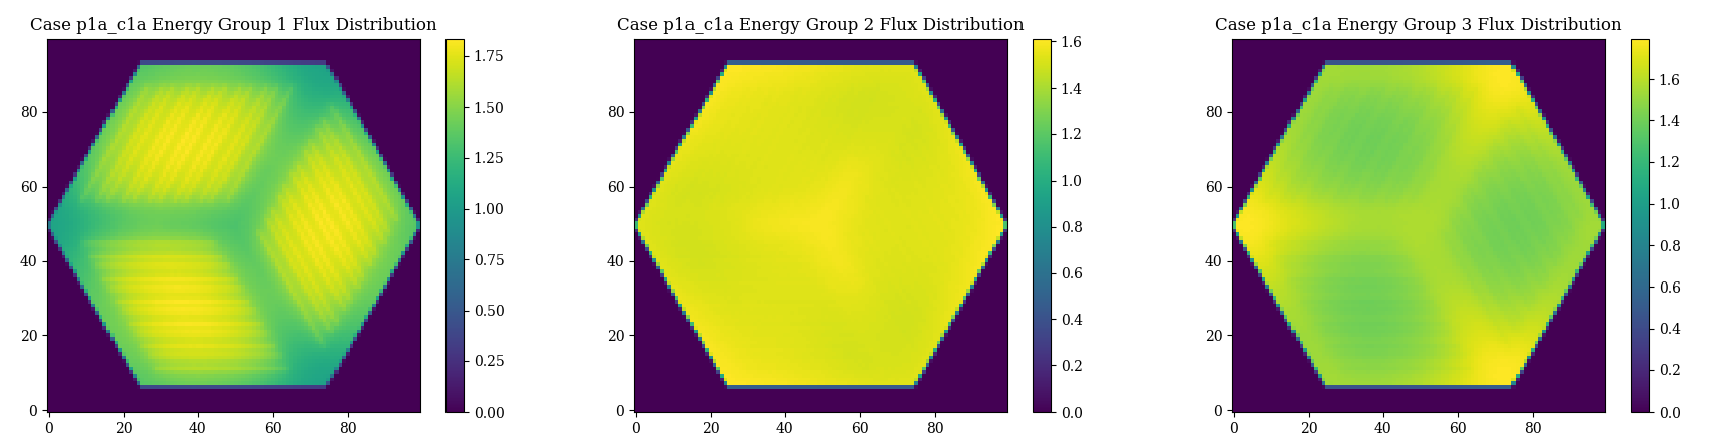
\includegraphics[width=0.9\linewidth]{phase1a-e-c1a.png} 
    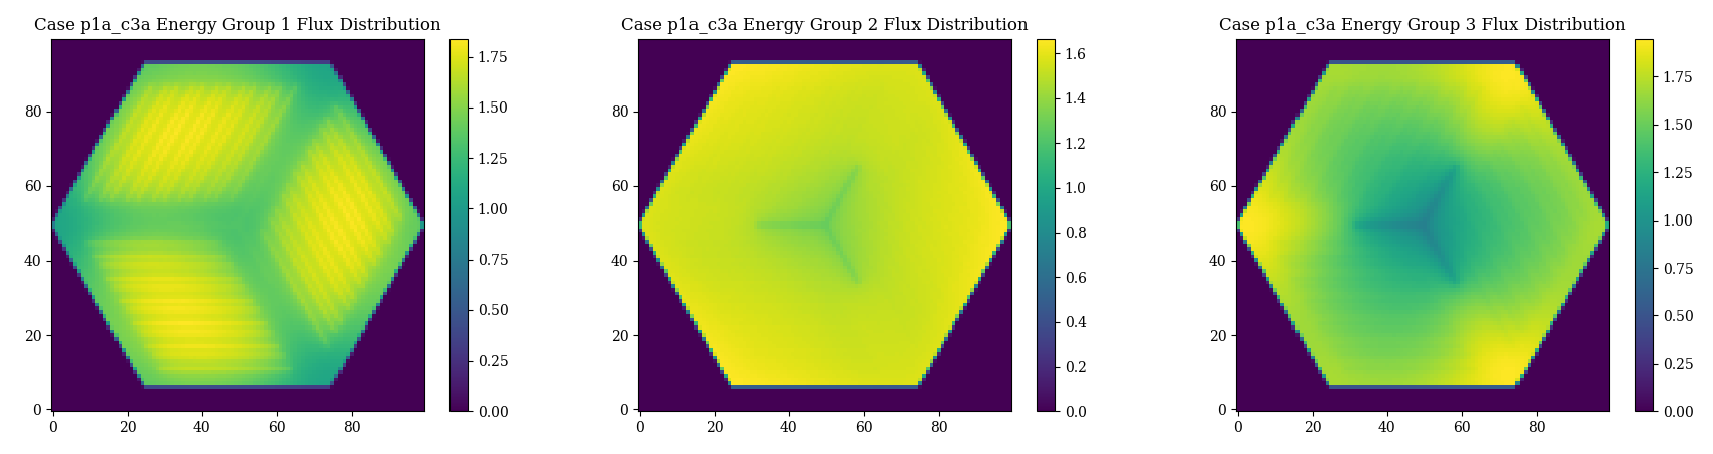
\includegraphics[width=0.9\linewidth]{phase1a-e-c3a.png} 
    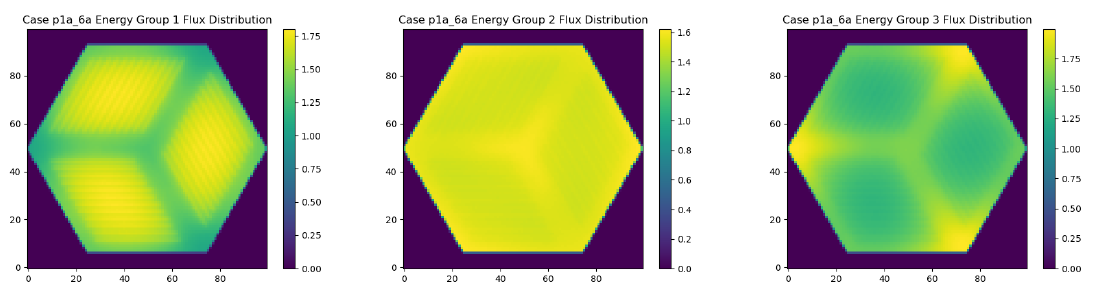
\includegraphics[width=0.9\linewidth]{phase1a-e-c6a.png} 
    \caption{\acrlong{FHR} Benchmark's Neutron flux distribution in 100 
    $\times$ 100 mesh for three coarse energy groups: Case 1A (above), Case 3A 
    (middle), Case 6A (below). Energy group 1: $E > 0.1$ MeV, Energy group 2: 
    $3 \times 10^{-6} < E < 0.1$ MeV, Energy group 3: $E < 3 \times 10^{-6}$ MeV. }
    \label{fig:phase1a-e}
\end{figure}
For all three cases, fast-flux peaks in the diamond-shaped sectors containing 
the fuel stripes, whereas thermal flux peaks outside of the diamond-shaped 
sectors. 
This is attributed to fission occurring at thermal energies in the 
fuel stripe area. 
For Case 3A, the thermal and intermediate neutron flux is depressed in the fuel 
assembly's control rod region.  
Case 6A has an increased heavy metal loading, resulting in a more pronounced 
fast-flux peaking and thermal flux dip in the fuel stripe area. 

Figure \ref{fig:phase1a-f} shows the neutron spectrum for Cases 1A and 6A. 
\begin{figure}[]
    \centering
    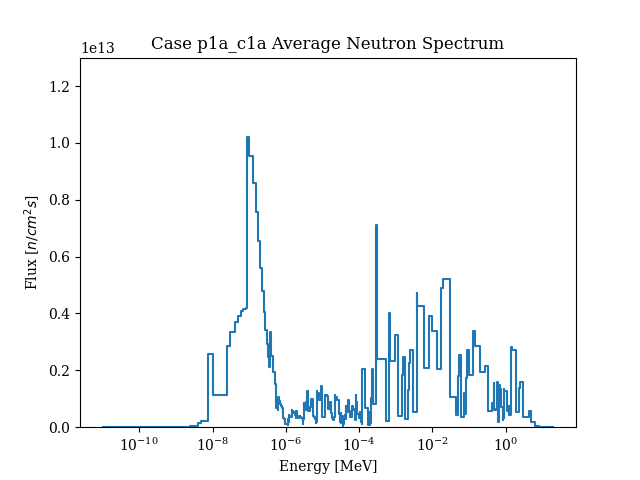
\includegraphics[width=0.49\linewidth]{p1a_c1a_f.png} 
    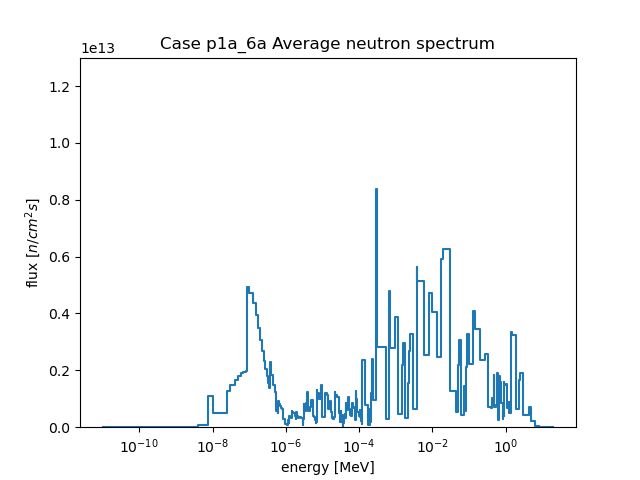
\includegraphics[width=0.49\linewidth]{p1a_c6a_f.png} 
    \caption{Neutron spectrum for \acrlong{FHR} Benchmark's Phase I-A Case 1A 
    (left) and Case 6A (right).}
    \label{fig:phase1a-f}
\end{figure}
Case 7A has a similar neutron spectrum as Case 6A since both cases have 
higher fuel content. 
All other cases have a similar neutron spectrum to Case 1A.
The neutron spectrum is faster for Case 6A and Case 7A due to more heavy metal 
loading and higher enrichment, respectively.  

\subsection{Results: Phase I-B}
Figure \ref{fig:phase1b_keff} shows the $k_{eff}$ evolution during depletion 
for Cases 1B, 4B, and 7B.
\begin{figure}[]
    \centering
    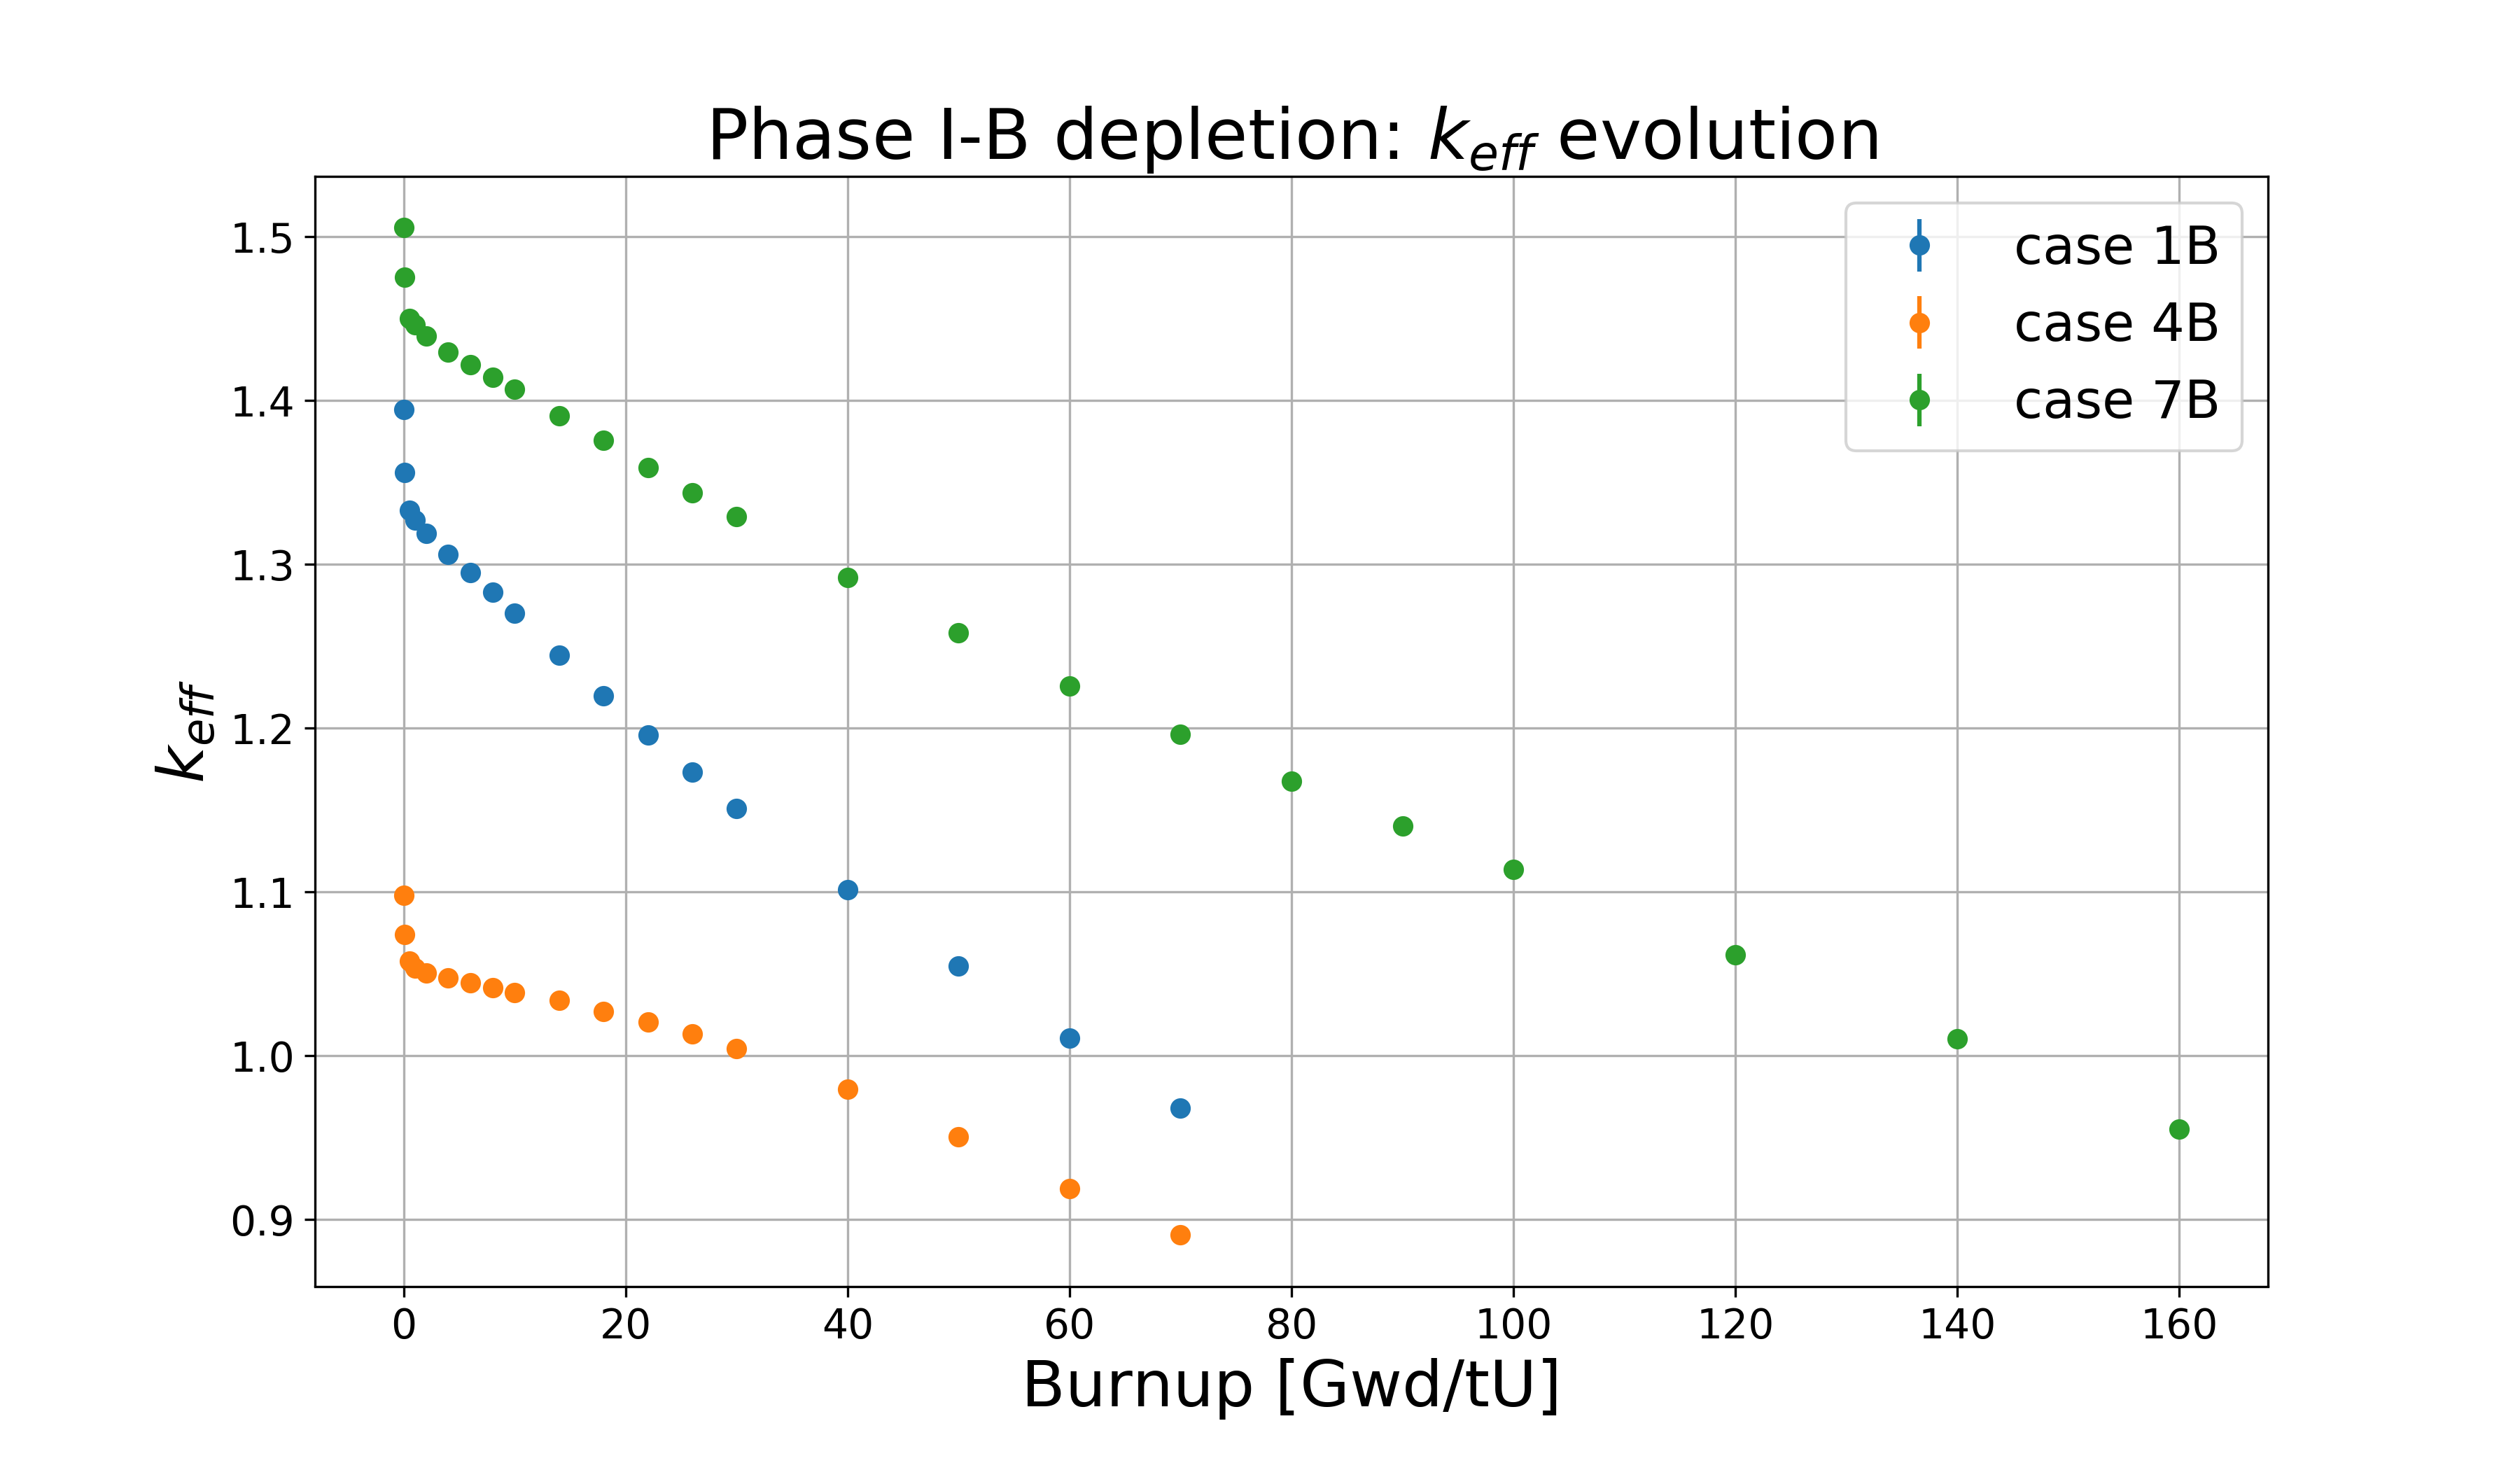
\includegraphics[width=\linewidth]{phase1b_keff.png} 
    \caption{\acrlong{FHR} Benchmark's Phase I-B depletion $k_{eff}$ evolution 
    for Cases 1B, 4B, and 7B. Case 1B is the reference case, Case 4B is the 
    discrete \gls{BP} case, and Case 7B is the 19.75$\%$ enrichment case. 
    Error bars are included but are barely visible due to the low uncertainty 
    of $\sim$40pcm.}
    \label{fig:phase1b_keff}
\end{figure}
The $k_{eff}$ at zero burnup corresponds to each case's 
corresponding Phase I-A $k_{eff}$ value reported in Table \ref{tab:phase1a-results}. 
Case 1B is the reference case with $9\%$ fuel enrichment and no \glspl{BP}. 
Case 1B's $k_{eff}$ steadily decreases until it reaches 0.967845 at the final 70 
GWd/tU burnup. 
Case 4B includes burnable poisons resulting in a lower initial $k_{eff}$. 
Its $k_{eff}$ decreases at a slower rate in the beginning due to the presence of 
burnable poisons, which decreases flux in the core. 
At approximately 20 GWd/tU, $k_{eff}$ begins decreasing at a faster rate, assumedly
due to burn-up of the poison material.   
Case 7B has a $19.75\%$ fuel enrichment, resulting in a higher initial $k_{eff}$. 
With a higher enrichment, the fuel can achieve a final burnup of 160 GWd/tU. 

\section{Summary}
% more enrichment / more HM does not mean higher keff, there is shielding 
% effects, thus, this leads us to believe that the phenomena is not as expected. 

This chapter described the \gls{FHR} benchmark specifications, \gls{AHTR} design,
and Phase I-A and I-B results obtained by the UIUC team. 
The benchmark results highlight the \gls{AHTR}'s passive safety behavior with 
negative temperature coefficients. 
Results such as a lower $k_{eff}$ for the \gls{AHTR} configuration with 
higher heavy metal loading demonstrated how increased fuel packing does not always 
correspond with increased $k_{eff}$ due to self-shielding effects.
These results hint at the possibility of minimizing fuel required by optimizing 
for inhomogeneous fuel distributions within the core. 
This will be further explored in the later chapters. 

